%
% 公立はこだて未来大学卒業研究中間報告書[全コース対応版]
%
%         ファイル名:"sample.tex"
%
\documentclass[11pt]{ujarticle}
\usepackage{funinfosys}
\usepackage{url}
\usepackage[dvipdfmx]{graphicx}

\author{% 
1020259 中村碧\\指導教員 : 松原克弥
}
\course{Intelligent Systems Course}

\title{Wii Fit BoardとSphero SPRK+による直感的なロボット制御のためのMROS2の活用}
\etitle{}
\eauthor{Aoi Nakamura}
\abstract{ロボットソフトウェア開発において,ROS(Robot Operating System)の利用が増えている。ROSはクラウドサーバと連携し,分散型ロボットシステムを構築するのに役立つ。しかし,各機能モジュール(ノード)の配置はシステム稼働前に決定する必要があり,予測困難な状況変化で最適なノード配置が変わる可能性がある。クラウドとロボット間でのCPUアーキテクチャの違いにより,稼働中のノードの再配置は技術的に難しい。
\\この研究では,ROSノードの動的配置機構の実現に向けた,組み込みデバイス向けROS 2ランタイム実装であるmROS 2-Posixを評価する。mROS 2-PosixがROS 2と比較してマイグレーションに優位性があるかを明らかにし,動的配置機構の実現への影響を実験結果で示す。
}
\keywords{ロボティクス,mROS2}
\eabstract{
\\}
\ekeywords{Roboethics, mROS2}
\begin{document}
\maketitle
%\vspace*{-.5cm}

\section{背景と目的}
さまざまな産業向けやエンターテイメント関連のロボットシステム,自動車の自動運転技術やIoTシステムの構築においても,これらのソフトウェア開発をサポートするフレームワークとしてRobot Operating System(以下,ROS)の普及が増加している[1]。ROSのプログラミングモデルは,システムの各機能を独立したプログラムモジュール(ノード)として設計することにより,汎用性と再利用性を向上させて,各機能モジュール間のデータ交換を規定することで,効率的かつ柔軟なシステム構築を可能にしている。たとえば,カメラを操作して周囲の環境を撮影するノード,画像からオブジェクトを識別するノード,オブジェクトのデータを基に動作制御を実行するノードを連携させることで,自動運転車の基本機能の一部を容易に実装できる。
\\ ROSのプログラミングモデルは,ロボット/IoTとクラウドが協力する分散型システムにおいても有効である。ロボットシステムのソフトウェア処理は,「センサー」「知能・制御系」「動力系」の3要素に分けられる[2]。クラウドロボティクスにおいて[3],主に知能・制御系のノードを高い計算能力を持つクラウドに優先して配置することで,高度な知能・制御処理の実現を促進し,さらに,必要な情報をクラウドに集約・保存することで,複数のロボット間での情報共有と利用を容易にする。
一方で,現行のROS実装においては,各ノードの配置をシステム起動時に設定する必要があり,先述のクラウドロボティクスのクラウドとロボット間の最適なノード配置を事前に設計する必要がある。しかし,実際の環境で動作するロボットは,ネットワークの状況やバッテリー残量の変動など,システム運用前に予測することが困難な状況変化に対応する必要があり,設定したクラウドとロボット間のノード配置が最適でなくなる可能性がある。このような状況変化に対する対応として,ノードを動的に再配置するマイグレーション機能の実現が求められているが,多くの場合でクラウドとロボット間のCPUアーキテクチャが異なり,実行中のノードをシステム運用中にマイグレーションすることは技術的に困難である。
\\ 菅らは,WebAssembly(以下,Wasm)を用いることで,クラウドとロボット間での実行状態を含む稼働中ノードを動的にマイグレーションする手法を提案した[菅さんの論文].
課題として,ROS 2をWasm化したことでオーバーヘッドが増大し,マイグレーション後,ノードの実行時間が大幅に増えてしまう問題が残った.
柿本ら[]は,組込みデバイス向けROS 2ランタイム実装であるmROS 2-POSIXを採用し,ROSランタイムのWasm化にともなうオーバヘッド増加に対処した.
しかし,採用されたmROS 2-POSIXはごく小規模なアプリケーション上でしか評価実験は行われておらず,今後もmROS2 POSIXを採用していく上でアプリケーションの規模を増加させた評価実験は必要不可欠である.
\\ 本研究では,クラウドとロボット間での実行状態を含む稼働中ノードの動的マイグレーションの実現に向けたmROS 2-Posixの評価を行い,mROS 2がROS 2と比べて動的配置機構の実現のソフトウェア基盤としてどの点で優位性があるのか明らかにすることを目指す.
%目的



\section{mROS2-POSIX}
 そもそもmROS 2[4]は高瀬らが研究開発を進めているROS 2ノードの軽量実行環境である.
mROS 2は中規模の組込みデバイス上で実行されるプログラムについて,汎用デバイス上のROS 2ノードと自律的に通信する機能を提供している.
このソフトウェア基盤によって,分散型のロボットシステムへの組込み技術の導入が促進できる.
組込みデバイスは計算資源が限定的であるが,これを活用することによってリアルタイム性の向上および消費電力の削減を図ることができる.
そして,mROS 2がPOSIX[]に対応したのがmROS 2-POSIXである.
本章では,組込みデバイス向けの高校率なROS 2通信方式およびメモリ軽量な実行環境を提供しているmROS 2-POSIXについて,ソフトウェア構成を中心に解説する.
\\ 図1(a)は,mROS 2-POSIXのソフトウェア構成を示している.上層から順に,まずmROS 2-POSIXアプリケーション層は,ユーザが実装するROS 2ノードに相当する.
\begin{figure}[h]
	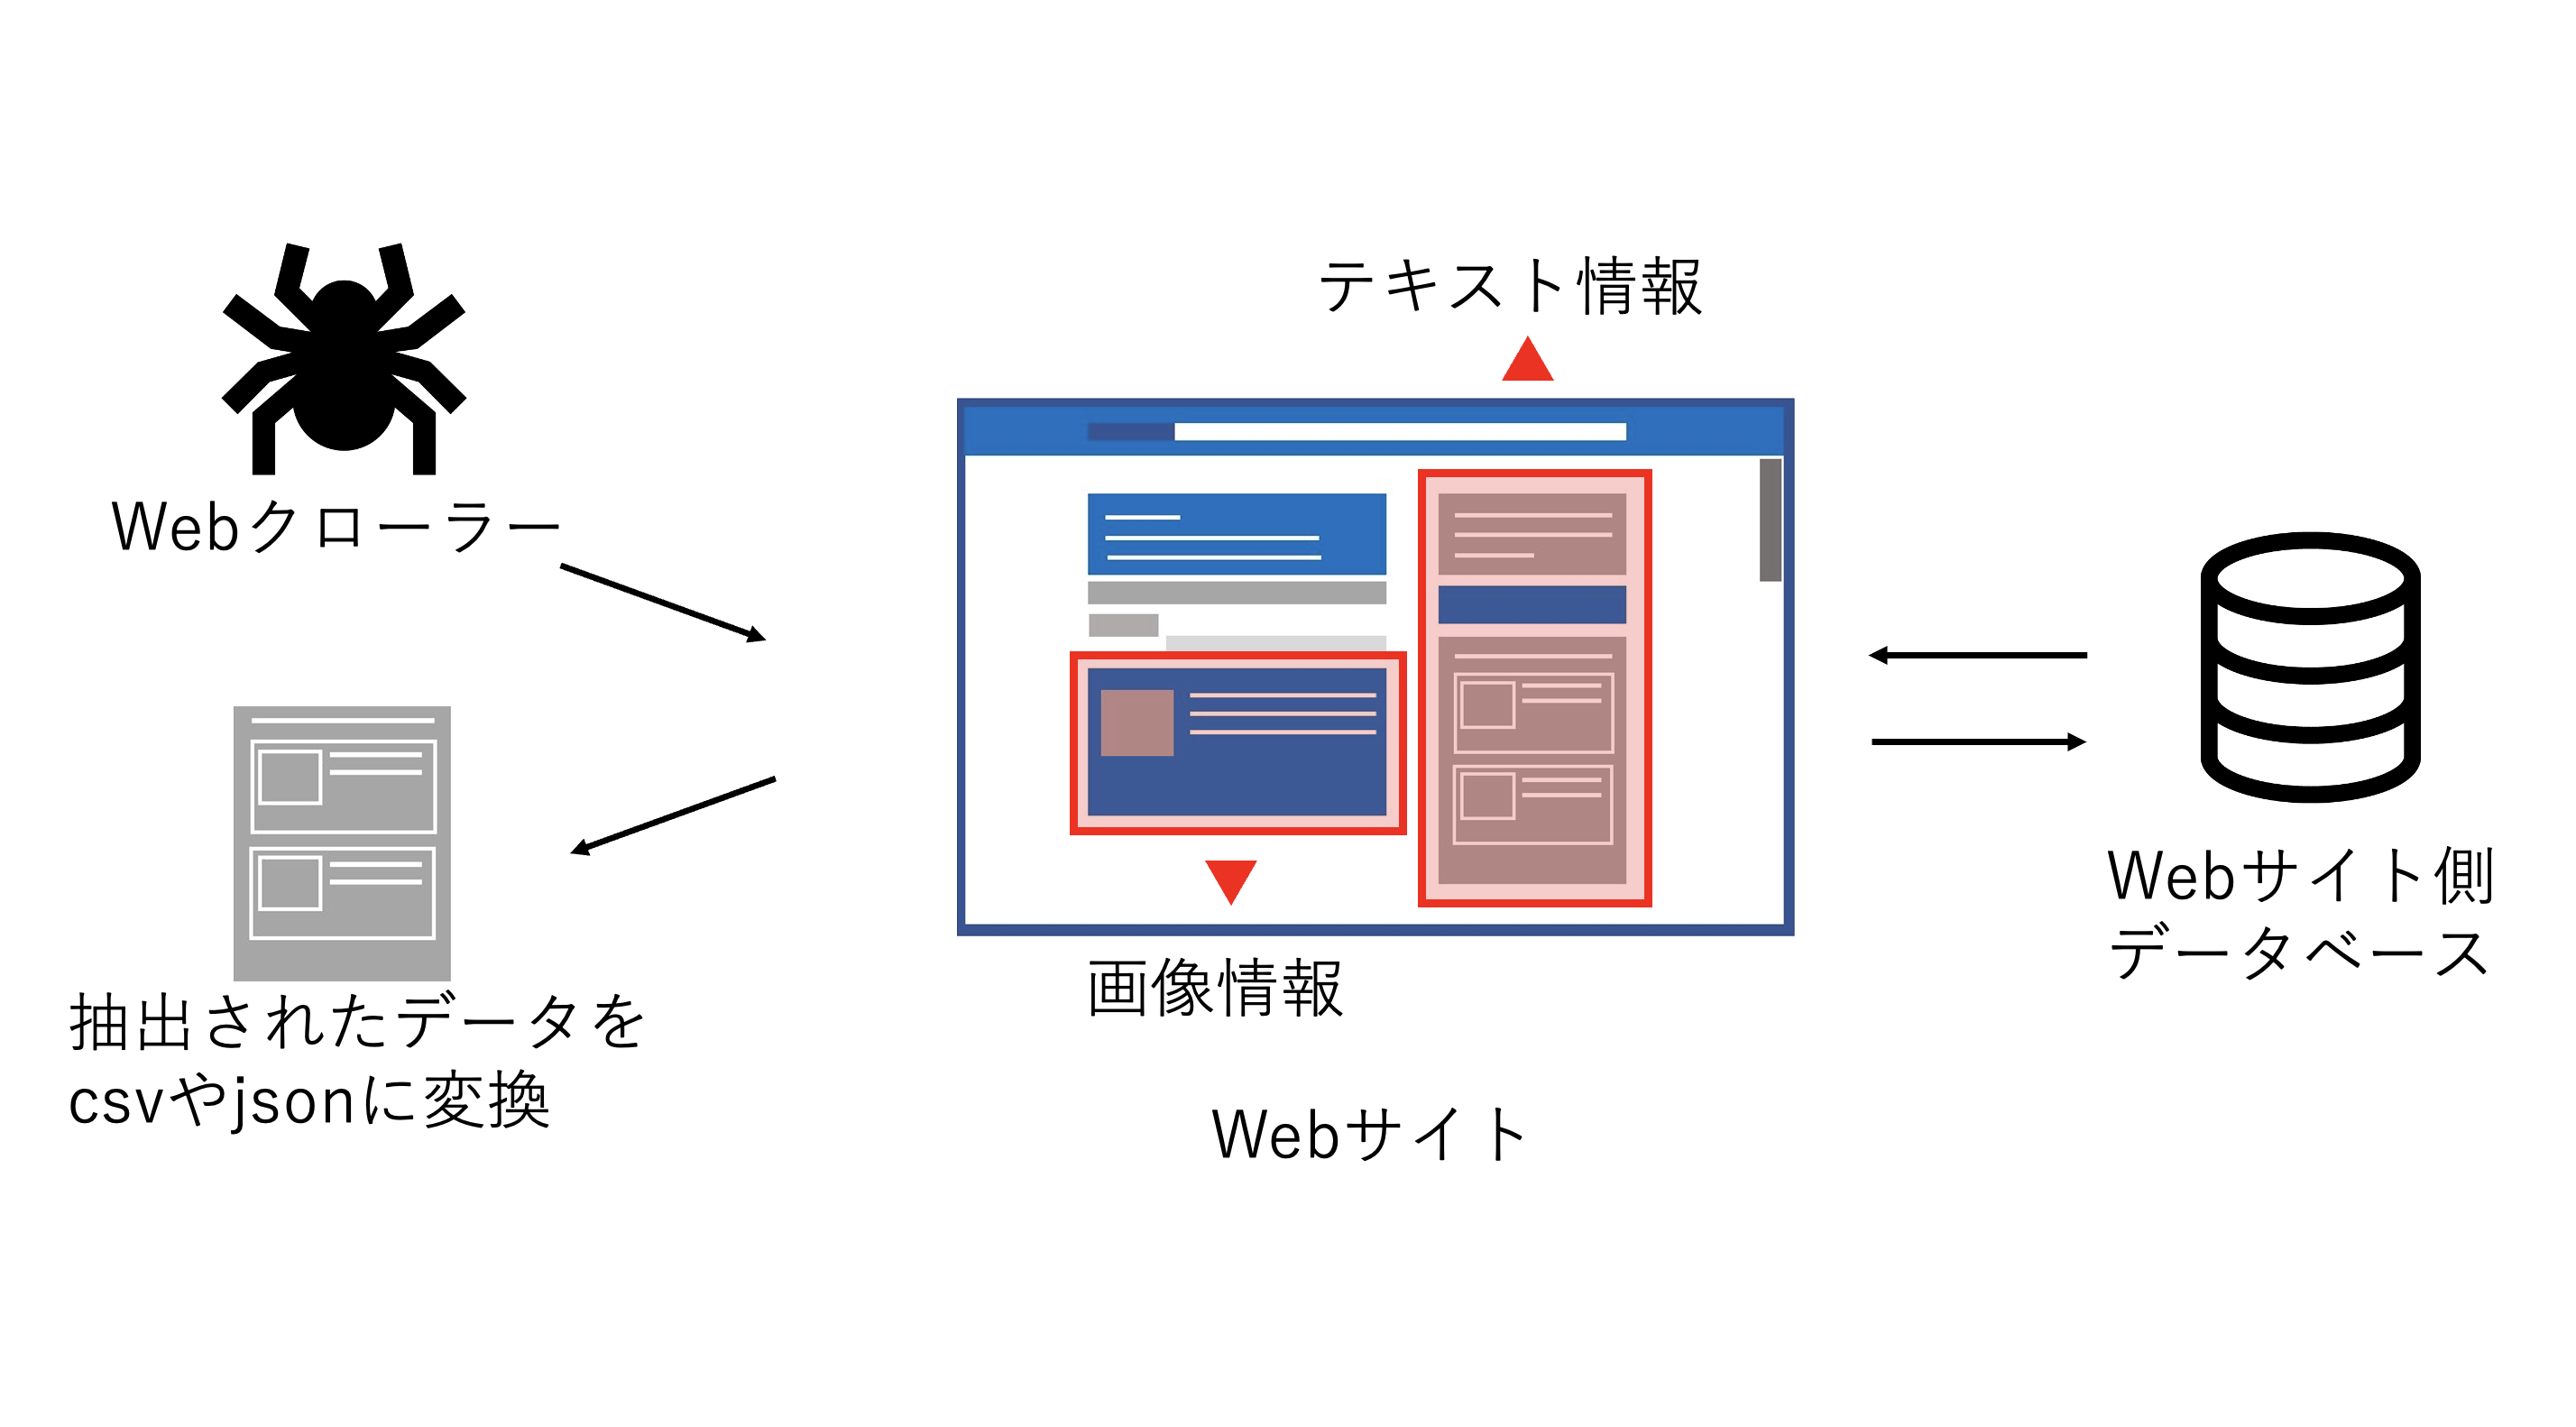
\includegraphics[width=0.9\linewidth]{./src/selenium.png}
	\caption{mROS 2とmROS 2-POSIXの内部構造}
  \label{fig:arch}
\end{figure}
mROS 2-POSIX API層および通信ライブラリ層は,ROS 2のtopicに相当するAPIおよび通信機能を提供する階層である.
本階層は,ROS 2のネイティブなクライアントライブラリであるrclcppと互換性を保つように設計している.
なお,mROS 2通信ライブラリでは,rclcppのうちpub/sub通信の基本的な機能のみ実装されている.
利用可能な機能は制限されているものの,組込み技術を導入するROS 2開発者は,汎用OS向けのプログラミングスタイルを踏襲しながらC++によってmROS 2のアプリケーションを実装することができる.
\\ Real Time Publish-Subscribe(以下,RTPS)プロトコルスタックにはC++実装のembeddedRTPS[]が採用されている.
メモリ領域の静的確保など組込みデバイスでの稼働を想定して設計されており,RTPSにおけるSimple Participant Discover Protocol(以下,SPDP)およびSimple Endpoint Discover Protocol(以下,SEDP)が実装されているため,通信の自立性が実現できる.
UDPについては組込み向けのC実装であるlwIP[]が採用されている.また,これらの階層はCMSIS-POSIX(Cortex Microcontroller System Interface Standard Portable Operating System Interface) APIに依存している.
通信層のembeddedRTPSおよびlwIPはCMSAIS-POSIXに依存しており,図1(b)に示すmROS 2のCMSIS-RTOS[]を互換した層になっている.
最下層にはハードウェアを抽象化したライブラリがある.
\\ mROS 2-POSIXの実行方式は,mROS 2が対応しているリアルタイムOSとの相違がある.
リアルタイムOSでは,組込みマイコンを実行資源の管理対象として,タスク単位でアプリケーションが実行される.
POSIXにおいてはタスクに相当する概念はプロセスであり,そこから生成されるスレッドを実行単位として処理が進行している.
\\ したがって,mROS2-POSIXは図2に示す実行方式を採用している.
\begin{figure}[h]
	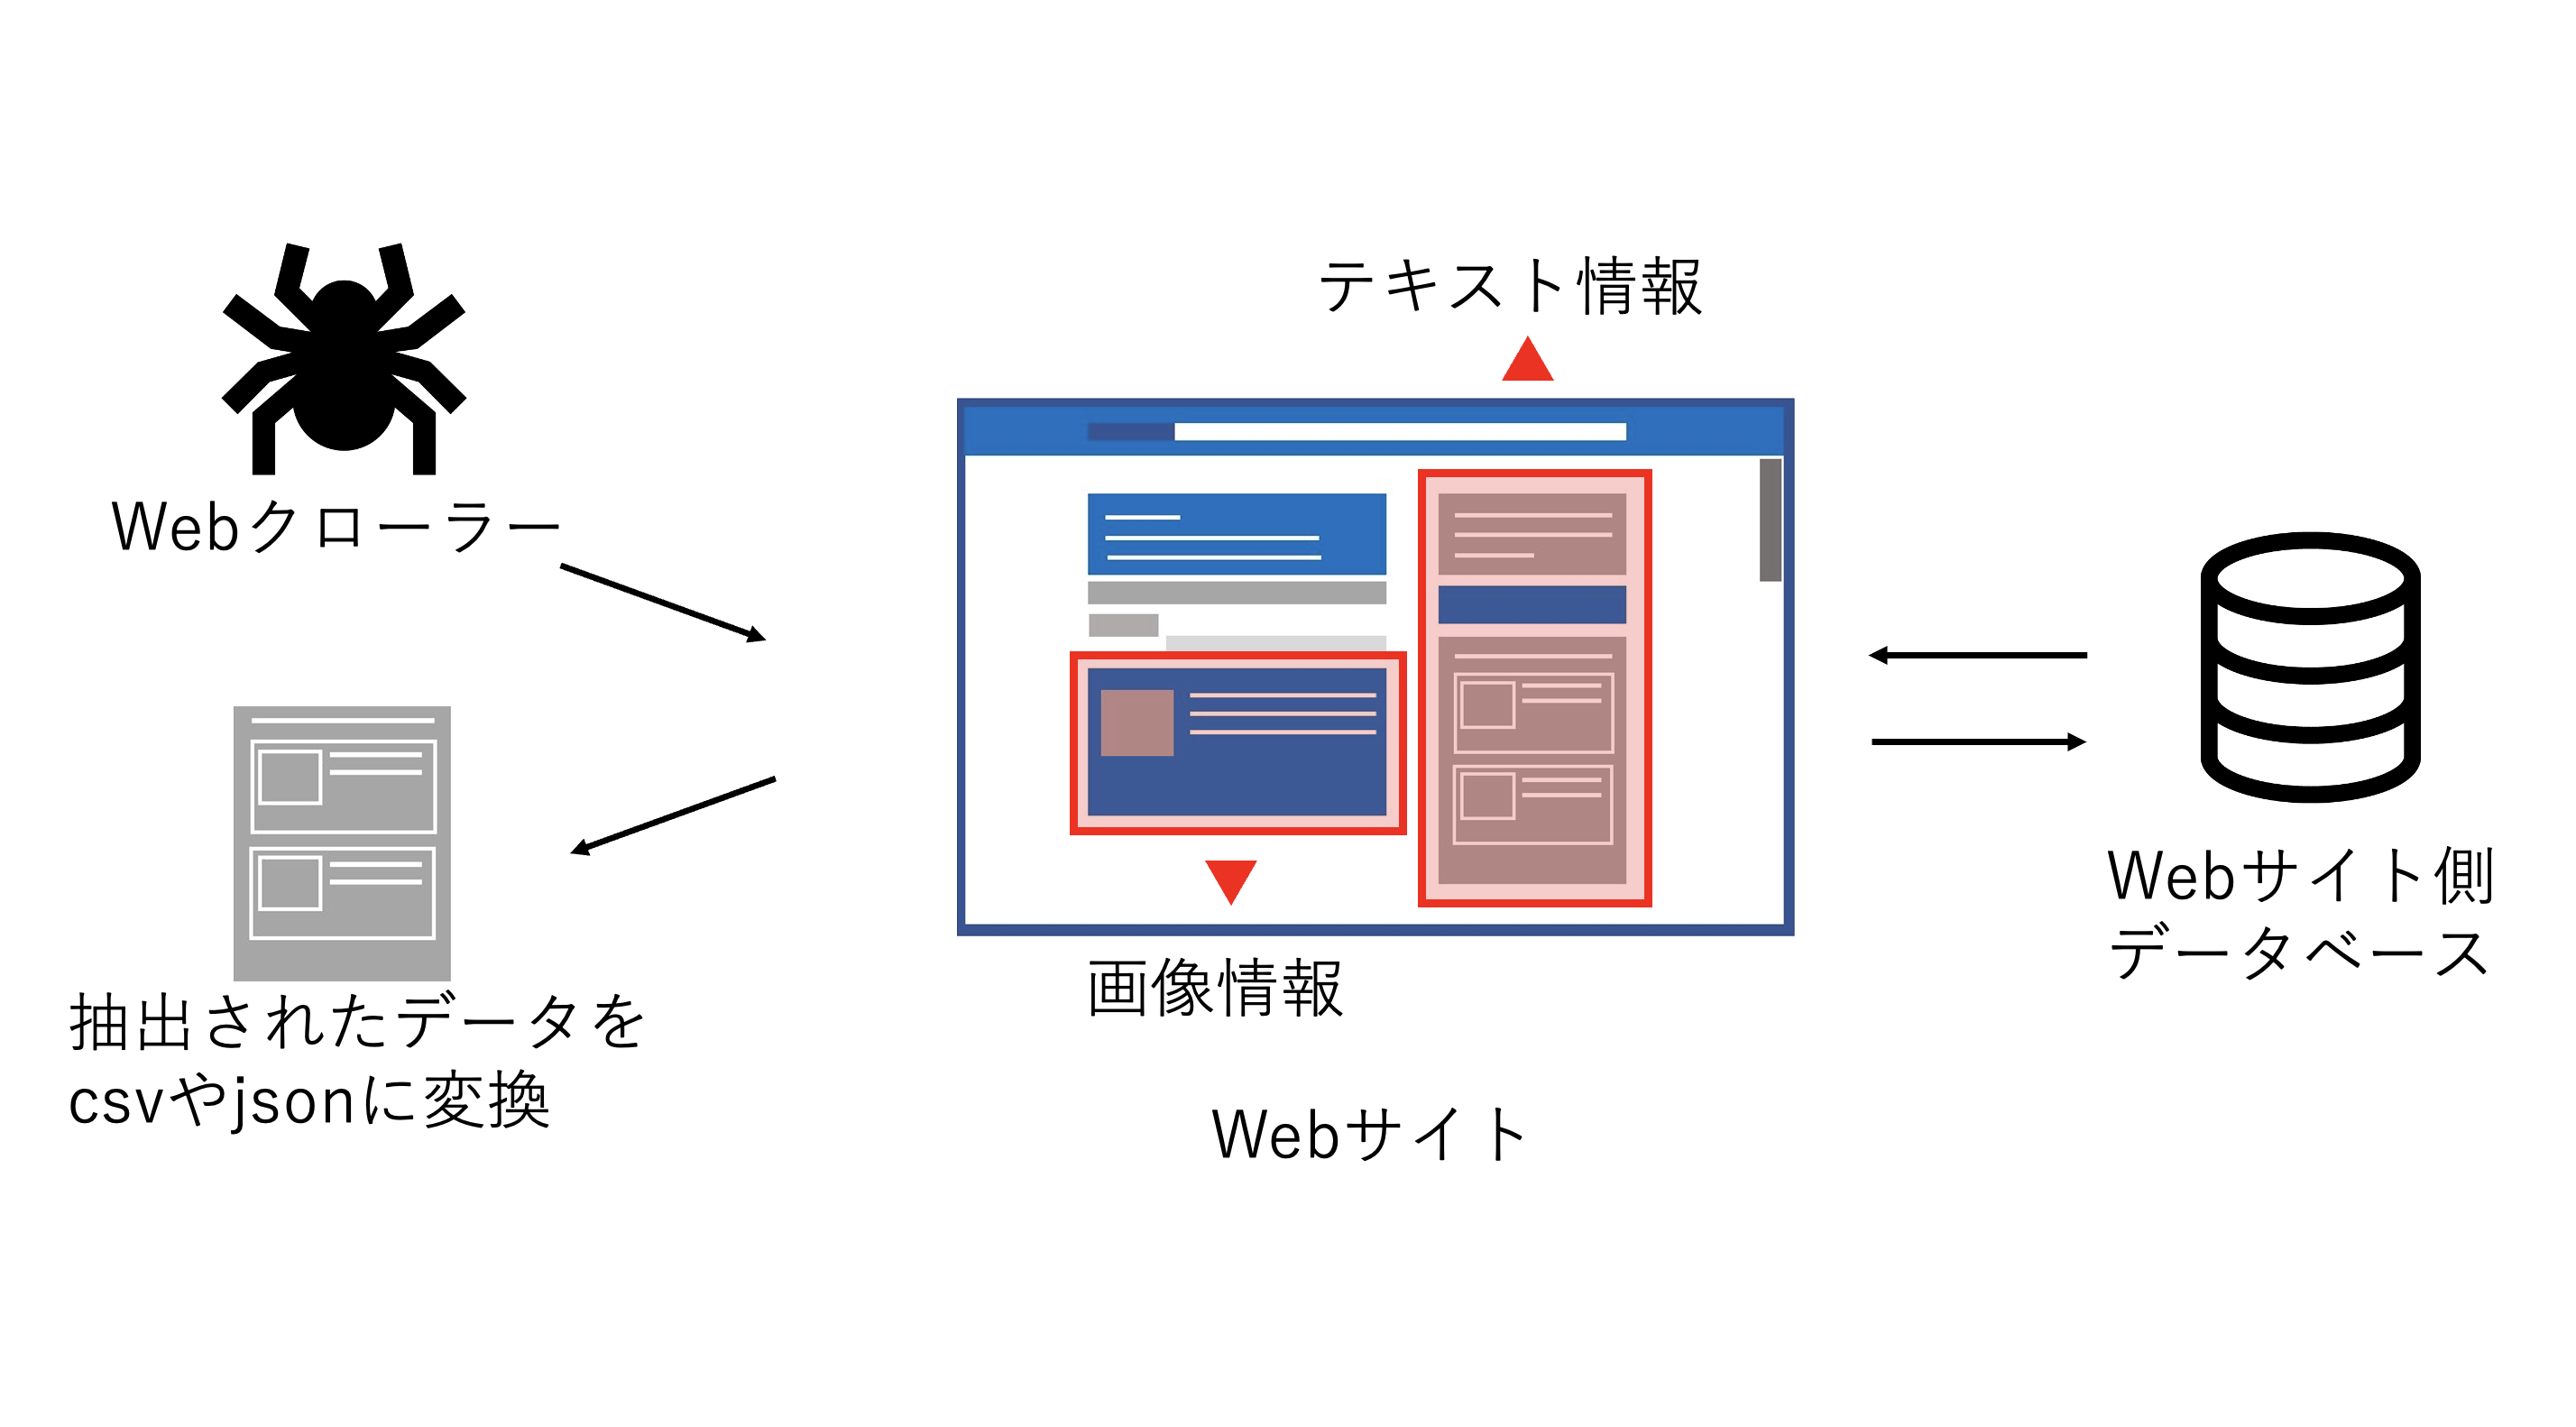
\includegraphics[width=0.9\linewidth]{./src/selenium.png}
	\caption{mROS 2-POSIXの実行方式}
  \label{fig:arch}
\end{figure}
mROS 2-POSIXの実行単位であるノードはPOSIXのスレッドに対応付けらており,mROS 2の通信ライブラリ機能を担う実行資源はPOSIXのプロセスとして捉え,これを管理対象としている.
組込みマイコンでの通信処理におけるイベント割込みについては,POSIX準拠OSにおけるブロッキングAPIの発行に相当させて処理されている.
\\ mROS 2とmROS 2-POSIXの機能構造の対応として,タスク管理機能は,スレッドの生成や開始などのPOSIX資源の管理機能に対応付けれている.
メッセージキューおよびミューテックスによるスレッドの同期・通信および排他制御は,POSIXではPthreadによって対応している.
メモリ管理機能はAlloc/Freeで,時間管理はOS時刻管理機能で対応している.
lwIPにおけるUDPパケット処理は,POSIXにおけるOS資源の操作に関する機能で実現されている.


\section{評価方針}
 mROS 2-POSIXを評価するにあったって,mROS2と同様のアプリケーションをROS 2に実装し,比較評価する.
mROS 2は,ROS 2のネイティブなクライアントライブラリであるrclcppと互換性を保つように設計されており,ROS2に同様のアプリケーションを実装した場合でも期待される動作をすることができる.
評価に使用するアプリケーションはWii Fit BoardとSphero SPRK+を用いたロボット制御アプリケーションである.
アプリケーションは,Wii Fit Boardはユーザの体重移動を検知し,Sphero SPRK+を前後左右に動かすことで,ユーザの体重移動に追従するように動作する.
図3にアプリケーションの構造を示す.
Wii Fit Boardに乗っているユーザの座標をパブリッシュするノードであるpublisher_wiiboardと,wiiboardというトピックにサブスクライブし,受け取った値をもとにSphero_SPRK+を動作させるwiibaord_sphero_sprkの2つのノードにわけられる.
このノードはそれぞれC++で実装されている.
評価項目としては,mROS 2-POSIXがROS 2と比べてどの点で優位性があるのかを明らかにするため,以下の項目を設定した.
\begin{itemize}
	\item 通信性能の評価
	\item メモリサイズの評価
\end{itemize}
 通信性能の評価については,1回の通信をロボットがLEDを点灯するまでの時間とし,それを100回行い,その平均と最大値と最小値と標準偏差を取ることで性能比較を行う.
\\メモリサイズの評価については,アプリケーションのバイナリをsizeコマンドで計測しそれぞれtext,data,bssのサイズを比較する.
\section{評価アプリケーションの実装}


\section{進捗と計画}


\section{結言}


\section{関連研究}


\section{知能システムコースにおける本研究の位置づけ}


\begin{thebibliography}{99}
	\bibitem{rikkyo}
	立教大学, "立教大学シラバス検索システム", 立教大学. [Online]. Available from: \url{https://www.rep-rikkyo.com/class_rooms?day=c&hour=4}. Accessed: 2023-10-25.
	\bibitem{gakugei}
	東京学芸大学 (非公式), "東京学芸大学教室検索システム", 東京学芸大学. [Online]. Available from: \url{https://u-gakugei-uoa.pages.dev/akitan/}. Accessed: 2023-10-25.
	\bibitem{selenium}
	SeleniumHQ, "Selenium Documentation", Selenium, 2023. [Online]. Available from: \url{https://www.selenium.dev/documentation/en/}. Accessed: 2023-10-25.
\end{thebibliography}
\end{document}
%
%
% EOF 
% \\ 図2.1(b)ではmROS 2のソフトウェア構成を示している.
% それぞれCMSIS-RTOS APIに依存しているため,mROS 2-POSIXはPOSIX APIとの差分を吸収する互換層(CMSIS-POSIX layer)を設け,通信を実現している.
% また,mROS 2は実行環境としてリアルタイムOSを採用していることに対し,mROS 2-POSIXではPOSIXに準拠したOS上でpub/sub通信を実現している.
% そのため,リアルタイムOSでは組込みマイコンを実行資源の管理対象として,タスク単位でアプリケーションが実行されるのに対し,POSIXにおいてタスクに相当する概念はプロセスであり,そこから生成されるスレッドを実行単位として処理が進行するという違いがある.
% mROS 2-POSIXでは,図2が示す
% は現時点で,TOPPERS/ASP3カーネル[]およびMbed OS 6[]を用いた実装が公開されている.
% Mbed OS 6は,CMSIS-RTOS APIのレイヤを標準的に備えている一方で,TOPPERS/ASP3カーネルはCMSIS-RTOS APIレイヤを備えていない.
% そのため,mROS 2ではTOPPERS/ASP3カーネル向けの実装として,それぞれのAPI差分を吸収するらっぽそうであるcmsis-asp3を用意して対応されている.
